\section{Deep Learning}\label{sec:deep-learning}

Deep learning method is part of machine learning methods based on artificial neural network with representation learning.
The learning process can be supervised, semi-supervised, or unsupervised.

There is a very large variety of deep learning architectures, some of them are specialized in some fields meanwhile others have a broader usage, especially, there are Convolutional Neural Network and Transformers.

\subsection{Convolutional Neural Network}\label{subsec:conv-neural-network}
The \gls{cnn} is a class of artificial neural network, it is used in almost every imagery related task, such as image classification, object detection, image segmentation, etc.

The CNN can take an input image, assign importance (learnable weights and biases) and process the input image by using the convolution operation extracting features.
\begin{figure}[H]
    \centering
    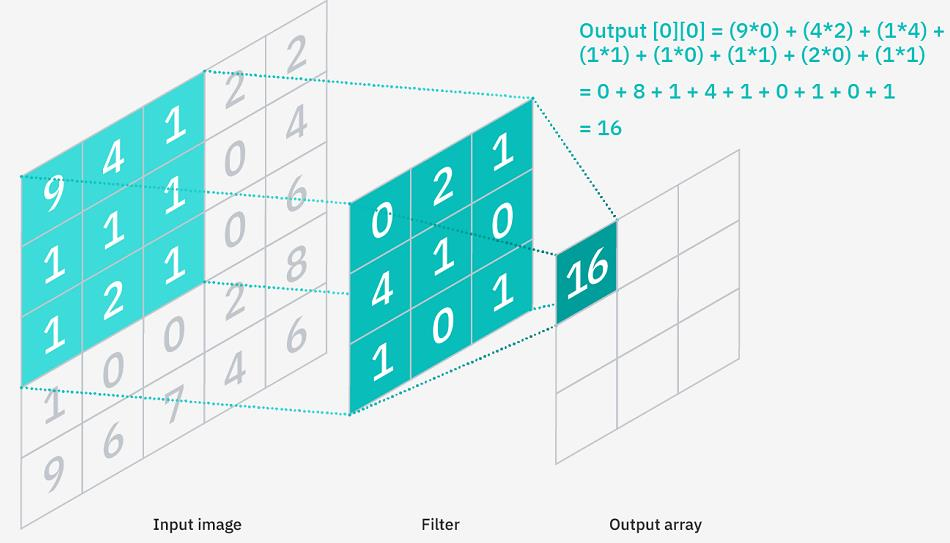
\includegraphics[width=\textwidth]{images/2_convolutions}
    \caption{Convolutions: every single element of the output feature map obtained summing the element-wise product between the elements from the input feature map and the kernel. The whole feature map is then obtained sliding the kernel over the input feature map.}
    \label{fig:convolutions}
\end{figure}
Increasing the number of layers and combining the pooling layers, the CNN is able to extract more and more complex features, such as edges, lines, shapes, etc.
The pooling layers, usually max-pooling and average pooling, can reduce the dimensionality of the feature maps, which is useful to reduce the computational cost.
For example, max-pooling is computed as showed in the image:
\begin{figure}[H]
    \centering
    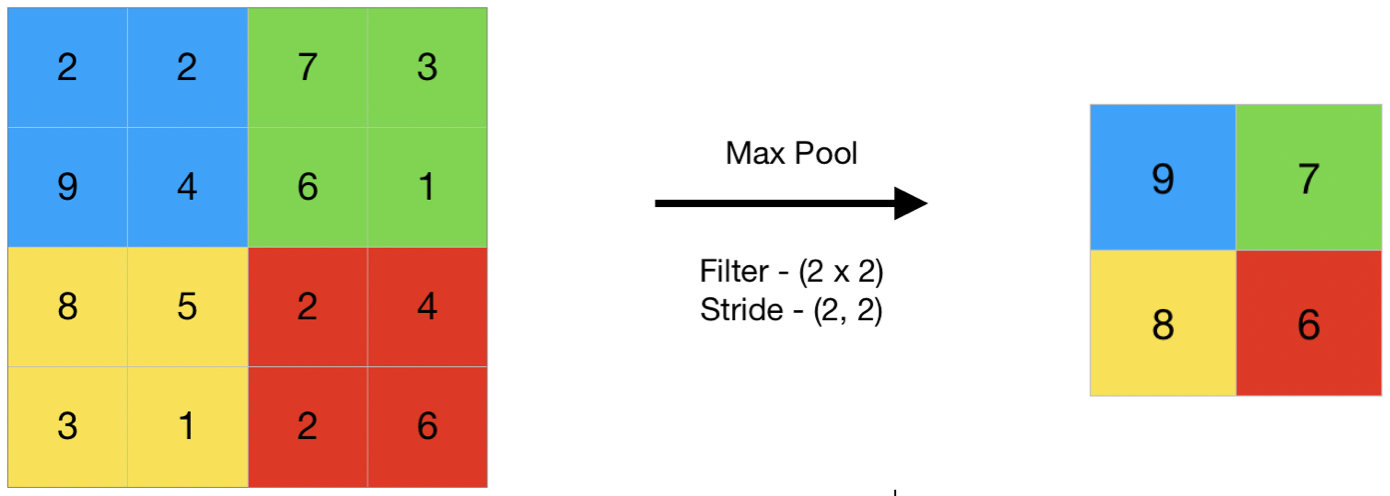
\includegraphics[width=\textwidth]{images/2_max_pooling}
    \caption{Max-pooling}
    \label{fig:max-pooling}
\end{figure}
With stride = 2, sliding over the input feature map and taking the maximum value of the window, the dimensionality of the feature map is reduced.
\subsection{Transformer}\label{subsec:transformer}
